\label{ch:impl}
This chapter presents the proposed implementation of the AHB system generator. Sec.~\ref{sec:hardover} provides an overview of the hardware described at the RTL. Sec.~\ref{sec:syslev} discusses how the ESL description is adapted to represent the hardware architecture. The challenges in creating a sound abstraction
of the hardware are elaborated. This is followed by an overview of the simulation models on both levels in Sec.~\ref{sec:sim}. The chapter is ended with Sec.~\ref{sec:results} where results of property checking and simulation times are presented.

\newpage
\section{Hardware overview}
\label{sec:hardover}
\begin{figure}[hbt]
    \begin{center}
        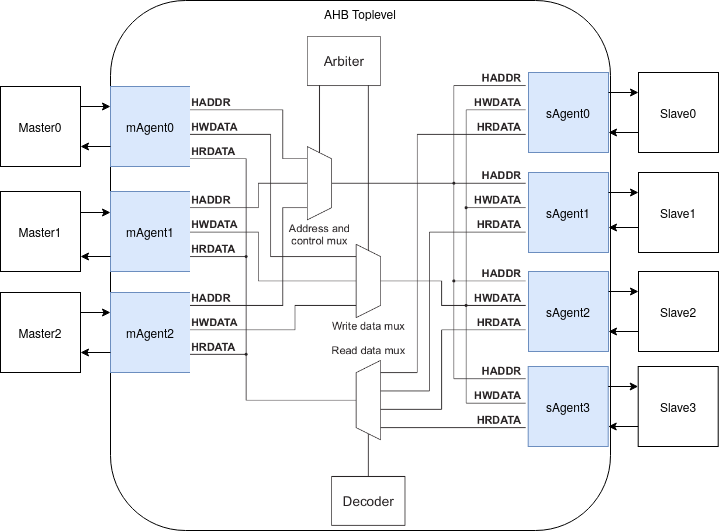
\includegraphics[width=0.8\textwidth]{figs/hw/Hw_toplevel.png}
    \end{center}
    \caption{Hardware top-level with 3 masters and 3 slaves connected}
    \label{fig:hw_toplev}
\end{figure}

For the purpose of this work, it makes little sense trying to implement the AMBA-AHB protocol from scratch starting at the ESL. It would take too much time to design the system and verify that it complies with the protocol. Instead, a trusted existing open source architecture is used. It is trusted in the sense that
it is often referenced when "the how" of protocol implementation is inquired. Furthermore, it has been available for scrutiny online for the last 15 years.  


\subsection{Existing hardware}
\label{sub:exist}
The existing hardware is taken from the \textit{ahb\_system\_generator} found at www.opencores.com \cite{ahbsys}. This architecture is already structured for the
means of generation and is implemented in VHDL, although is doesn't support wide data bus configurations it is the ideal candidate for this work. The master and slave agents was not taken from this source, they were rather redesigned to match SystemC-PPA compliant modules. This architecture supports fixed-priority, round robin and random priority arbitration. There are also modified versions of these arbitrations, where a grant is maintained as long as \textbf{HBUSREQx} is asserted. The chosen arbitration for this work is the modified fixed-priority. The possibility of starvation is a drawback, but it is far less complicated to model at the ESL than for example round robin. Due to limited time, burst, split and retry transfers are not implemented in the agents. The the modified extension to fixed-priority is selected to simplify an implementation of burst transfers. A study of this is presented in chapter \ref{ch:summary}. This hardware is represented in Fig.~\ref{fig:hardover} as the arbiter, decoder and wires connecting the agents. For simplicity it will collectively be referred to as the bus matrix. \par 
For reasons discussed in Sec.~\ref{sec:syslev} a property set was manually described to discover a suitable abstraction of this hardware. In the process it was
discovered that the default slave did not provide a zero cycle OKAY response when it was supposed to. It did however, provide the two cycle ERROR response as 
required by the protocol. This error does not change any functionality of the design, and would never show up in simulation unless a master or agent was sensitive to this. Because it complicated the development of a property set, it was corrected. 

   
\subsection{Master agent}
\begin{wrapfigure}[12]{l}{5cm}
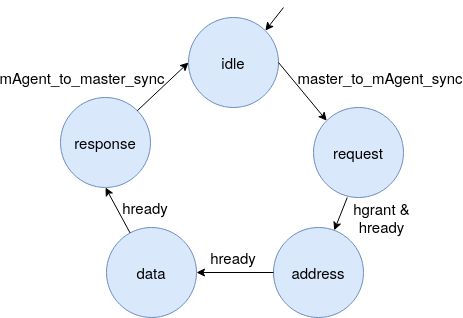
\includegraphics[width=5cm]{figs/hw/mAgent_FSM.png}
\caption{Master agent FSM}\label{fig:rafsm}
\end{wrapfigure}  

The master agent implements the master side of the AHB protocol. It is initialized to the \textit{from\_master} state, where it awaits a payload. The $agent\leftrightarrow master$ interface implements the four phase handshake in both directions. In other words, it is blocked pending a a synchronization signal from the master. The payload represents only a subset of the AHB master interface. The remaining signals are hardwired to default values. \textbf{HTRANS} is an exception, this signal is controlled by the agent throughout the transfer. In an ESL description it is sometimes beneficial to use enums to represent certain encodings and signals. This is to enhance readablility for the designer. These enums have been directly transferred to the RTL description. The entire payload is listed in table \ref{tab:mpayload}, where unchanged signals are marked with a dash.  

\begin{table}[hbt] 
  \label{tab:mpayload}
  \begin{tabular}{|p{25mm}|r|p{10cm}|} 
  \hline
  \textbf{Signal} & \textbf{Type} & \textbf{Content} \\
    \hline
  \textbf{HADDR} & - & - \\
    \hline
  \textbf{HWDATA} & - & - \\
    \hline
  \textbf{HWRITE} & enum & AHB\_READ, AHB\_WRITE \\
    \hline  
\textbf{HSIZE} & enum & MT\_B (byte), MT\_H (halfword), MT\_W (word) \\
    \hline
  \end{tabular}
\caption{Master out payload}
\end{table}

The return payloads consists of only \textbf{HRDATA} and \textbf{HRESP}. A key drawback that is obvious from the FSM is that the agent will return a payload 
to the master regardless of transfer direction. Surely throughput would be higher if the agent bypassed this state in the case of a write. If the transfer
status is not reported back to the master, any error would only be known locally in the agent. It would be possible to assert an error signal that is checked 
before starting a new transfer. However, any predesigned code for a CPU using the AHB protocol i.e linux is likely to expect the error to apply to the current transfer, not the previous. To avoid limiting the bus to systems with manually tailored code, a payload is returned to the master in any case. This comes
at the cost of latency, but as discussed this is a reasonable trade-off. \par
An overview of a transfer is provided with respect to the FSM.
\begin{enumerate}
 \item \textit{from\_master}: Initial/idle state, when a synchronization signal is received, the payload is translated to pure bit and bit vector values and written to the AHB interface.
 \item \textit{Request}: \textbf{HBUSREQx} remains asserted until agent is granted the bus and the bus is ready.
 \item \textit{Address}: \textbf{HTRANS} is encoded with NONSEQ, signalling the start of a transfer. This remains encoded until the bus is ready.
 \item \textit{Data}: When the bus is ready, return payload is read from the AHB interface and written to the master.
 \item \textit{to\_master}: Agent waits for a synchronization signal from the master. The master should already be asserting its synchronization signal, but this is not a requirement.   
\end{enumerate}

The sequence of operations above does not seem to match the sequence in the protocol covered in Sec.~ref{sec:ahb} in the previous chapter. It is however, 
understood that address/control and data can have arbitrary values outside their respective phases, as long as the intended values are present in their 
respective phases. It is therefore also not an issue that they have the intended values outside the respective phases as well. This is provided that \textbf{HTRANS} have the correct encoding at all times.  \WKSAY{Specify that reads and writes are equal if this design desicion remains}
 

\subsection{Slave agent}
\begin{wrapfigure}{l}{5.5cm}
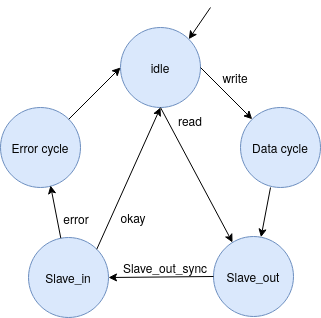
\includegraphics[width=5.5cm]{figs/hw/sAgent_FSM.png}
\caption{Master agent FSM}\label{fig:rsfsm}
\end{wrapfigure}  

The slave agent implements the slave side of the protocol. 

\WKSAY{I think this FSM is misleading, since HREADY=1 is part of the data phase}
As figure \ref{fig:rsfsm} shows the slave agent FSM is more complex than that of the master agent. To make the slave agent comply with the AHB protocol it needs to both obey the rules of the transfer phases and provide the proper response while communicating with its slave. A slave agent is always ready to receive a payload from its master, namely the AHB matrix. \WKSAY{the word phase should not be used for idle in slaves}
Starting from the \textit{idle\_phase} the agent stays idle until it is both selected and the encoding of \textit{nonseq} is detected on its inputs. When true it samples address and control signals from the AHB matrix and proceeds to the \textit{data cycle} where it samples the data. After sampling the data, the payload is written to the slave out port named \textit{sAgent\_to\_slave}. At this point the agent waits for a handshake, which should normally occur instantly but that is not a requirement. After the handshake is received it proceeds to wait for the response data and status from the slave, as with the output there is not a strict requirement on the wait time but it is recommended to keep the wait states under 16 cycles in total. The slave agent deasserts \textbf{HREADY} throughout its entire conceptual data phase, and zeroes \textbf{HRDATA} one clock cycle after asserting \textbf{HREADY}. \\
\newline
\WKSAY{this is highly misleading, it may not be operated by another master, only one can be operated at a time, rather it signals to the bus that it is not ready yet.}
The slave agent may at any given timepoint be operated by another master. This is why the slave deasserts its \textbf{HREADY} throughout its entire conceptual data phase. It is standard for a slave to introduce wait states. As with a DRAM module, there are delays associated with activating a row (insert data). As with DRAM this delay is minimized in sequential address transfers using bursts. In contrast to the diagram in figure \ref{fig:transfer}, the conceptual data phase of the slave agent does not include the assertion of \textbf{HREADY}. 
\WKSAY{what is a misnomer? and dont use the word assertion this way.}
This is a slight misnomer since the data phase does in fact include the assertion as seen from the properties. It is however not included in the FSM to not diffuse the differences between the states. The \textit{idle\_phase} and \textit{error cycle} only differentiate in the value of \textbf{HRESP}. Although the assertion of \textbf{HREADY} technically is a part of the data phase, it is however beneficial to highlight that these are separate states, as they are represented as such in the RTL description. The zeroing of \textbf{HRDATA} is a design choice to increase abstraction. \WKSAY{Why does this increase abstraction, this hangs a bit loose}
\newpage

\section{System level representation}
\label{sec:syslev}
\begin{figure}[hbt]
    \begin{center}
        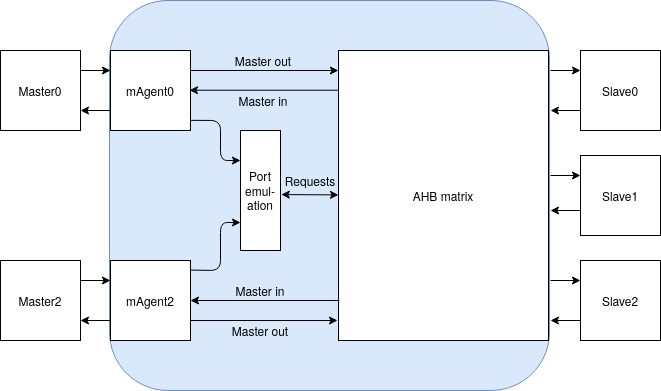
\includegraphics[width=0.8\textwidth]{figs/ESL/Syslev.png}
    \end{center}
    \caption{ESL toplevel with 2 masters and 3 slaves connected}
    \label{fig:esl_toplev}
\end{figure}

When representing the AHB system at the ESL, abstraction is a priority. Ideally there would be a single SystemC-PPA describing the entire system. It is on 
the other hand not possible to represent this multi-master design without separating the master agents into their own SystemC-PPA. The reason for this is 
parallelism, and a single threads lack of capability to represent it. Regardless of which conceptual state the system is in, any idle master can receive 
a message and proceed to request. This operation requires the modification of the output \textit{mAgent\_to\_master(x)\_notify} in addition to knowledge of this
request at the next conceptual system state. This is not practical to represent at the ESL, if it is even possible. Considering that the ESL needs to represent an existing RTL description, it is beneficial to manually write the properties bottom-up to get an idea of how the system level description must be formed.

\subsection{Manual property set}
During the development of the initial property it became clear that to determine the state of the bus, knowledge of past behaviour is required. It is not possible to determine only by observing the internal registers of the design. It is easy to determine which master owns the address and
data bus. However, this provides little information when the operating master is the default master. Even when observing the encoding on \textbf{HTRANS}, it is impossible to determine if the default master is active or idle in the data phase. One alternative is to look at past values of \textbf{HTRANS} to determine if the default master recently was in the address phase. Another much simpler alternative is to exploit that master agents are verified in separate clusters. The
state of the master agents are determined as outputs to their clusters and as inputs to the main cluster. The state of the bus is now possible to determine at any time by observing the states of the master agents. \par
The next steps in developing a complete property set include discovering visible registers and determining outputs to the design. Most of the important signals
in this design are updated on a clock edge, which is straightforward to represent at the ESL. One of the signals of the master interface, \textbf{HGRANTx} is 
not updated on a clock edge. This is problematic because it is not feasible to determine a fixed value for this signal in the next time point. \textbf{HGRANTx} 
must be updated with the output of a function. For the same reason, the signals on the address bus can not be represented directly. The visible registers 
representing the address bus are rather the inputs from the master agent in the state \textit{Address}, and if none apply a default value is selected. 

\subsection{Forming the ESL}
 




\WKSAY{Describe in detail the problem with multi-master designs, then describe in detail key things that must be represented in the ESL, like hready and hgrant in terms of the phases. They must be determined}
Describing the AHB system with SystemC-PPA in a single cluster is no longer feasible when more than one master is connected to the bus matrix. The master agents must be contained within their own clusters, or PPAs so that it does not need to be accounted for every possible combination. Since only one slave may be operated at a time, including them in the bus matrix PPA reduces the overhead. The interface between the master agent and the bus matrix have signals with mostly identical values for all masters, the exception is \textbf{HGRANTx}. This signal is purely combinational in the implementation, meaning that it changes its value within the same clock cycle as its initiator. Using any combination of existing ports there was not found any manner to represent this interface for multiple masters. The decision was made to create the properties bottom-up, to determine if the interface could be represented using existing ports and if not, where the gap is. Gap free verification was used for this purpose, with the style of generated properties in mind. 

\subsection{Bottom-up abstraction}
\WKSAY{bottom up properties}
The first challenge of carrying out the GFV process is determining the CSM of the AHB. It has to be represented in such a way that it is feasible to describe at the ESL. Looking at other formal verification efforts made on the AHB \cite{ahbformal}, it can be seen that the real FSM of an AHB is incredibly complex. 
\WKSAY{it is incredibly complex because of burst} Furthermore, it is described how the state of the bus is dependent not just on state and inputs but on previous states as well. It is necessary to know the state of the bus, namely if there is a transfer being carried out or not. It is not as simple as paying attention to bus ownership since there is no way of knowing if there is a transfer in progress when the default master owns the data bus, without looking at past values on \textbf{HTRANS[1:0]} \WKSAY{long and useless sentence, this whole thing should be rewritten}. One would furthermore need to constrain the design to establish how far into the past to look. One could go with the suggested maximum delay of slaves for 16 clock cycles. A much simpler solution is to define the master agents states as outputs to their clusters, and define this as inputs to the main cluster. By only concerning with which masters are requesting and where the data goes, the CSM can be made quite simple. If one was concerned with which master owned the address and which master owned the data bus at all times it would lead to state explosion, making an ESL description unfeasible even for a low number of masters.     

\begin{figure}[ht!]
	\centering
	\begin{minipage}[t]{0.49\textwidth}
		\centering
		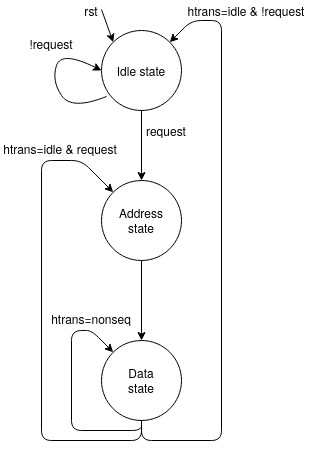
\includegraphics[scale=0.5]{figs/ESL/Bus_fsm_new.png}
		\captionof{figure}{Abstract CSM}
		\label{fig:OC}
	\end{minipage}
	\begin{minipage}[t]{0.49\textwidth}
		\centering
		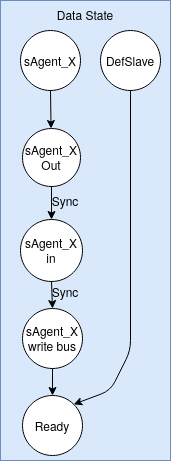
\includegraphics[scale=0.5]{figs/ESL/Data_state.png}
		\captionof{figure}{Detailed data state CSM}
		\label{fig:eslfsm}
	\end{minipage}
\end{figure}


By using a fixed priority arbitration scheme it is simple to determine which master is granted the bus. 
\WKSAY{This is nonsense, it needs to be restructured, be more descriptive, separate ESL states from property states}
By dividing the transfer into three main states with the data state divided into five further, there is no need to impose any constraints on wait states. The bus is ready (\textbf{HREADY} is set) at the end of each state and any request is ignored unless the bus is ready. The states can be defined as follows:
\begin{itemize}
\item Idle state: No transfer in progress.
\item Address state: One master is in the address phase of the transfer, no masters are in the data phase. There is no trigger for the next state as the bus/slaves will always be ready here. 
\item Data state: One master is in the data phase of the transfer. This state is broken down into five substates per slave, with default slave as exception.  
\end{itemize}


\WKSAY{This does not describe the bottom up properties, it describes the actual properties. you need to separate that}
It is worth noting that in the idle and address state the bus/slaves are always ready. The payload is transferred between the states using visible register which are named \textit{AS\_regs} for the address state and \textit{DS\_regs} for the data state. The Data state is divided into several important states to describe the transaction between the slave and its agent while simultaneously describing all necessary outputs. The default slave has only two states and they are self explanatory because of the two cycle error response. The remaining slave agents are explained by the following:
\begin{itemize}
 \item First state: There is one clock cycle delay required to allow the slave agent time to sample the possible data provided in the data phase.
 \item Second state: Slave agent writes payload to slave using blocking write. 
 \item Third state: Slave agent reads back from slave using blocking read.
 \item Fourth state: Slave writes payload back to bus. This requires two cycles due to the possibility of error, error cycle was removed from master agent due to inconsistencies in simulation. For this reason information on error is only contained within the visible registers handling response.   
 \item Fifth state: The bus is ready, payload is sampled, requests are handled and next state is determined based on the value of \textbf{HTRANS[1:0]}, which has been added to \textit{AS\_regs} alongside the payload. 
\end{itemize}

It is easy to see that the differentiation between read and write within the AHB matrix would lead to the double amount of data states \WKSAY{consider the trade-off, is it worth it?}, with the gain being one clock cycle saved in the case of a read \WKSAY{confusing and also probably wrong}. The entire design is represented by this CSM using only properties with length $t=1$ \WKSAY{t is the arbitrary timepoint, t=everything, use t\_end or something}so determining the output is straightforward with the exception of \textbf{HGRANTx}. As this is an output that is not stored in a register its value updates in the same clock cycle as its \WKSAY{is instrigator the word?} instigator. This is not a problem to model in the properties themselves, but this representation does not allow for any sound abstraction between the RTL and ESL \WKSAY{rather say it is not possible to represent by assigning value to a variable}. Determining the value of \textbf{HGRANT} in the next clock cycle is not feasible in this implementation. One would have to account for every \textbf{HBUSREQx} as an assumption at $t+1$ in every property. An alternative could be to enable this output through a register but this would lead to unpredictable behavior. This output is simply determined as the output of a function \textit{mx\_grant} and is at the ESL represented using an enum. \\
\newline
The design choice to zero \textbf{HRDATA} and modify the default slave response entails that \textbf{HRDATA} and \textbf{HRESP} will be zero unless it is in the fourth or fifth conceptual data state \WKSAY{this sentence is garbage}. After adding all determination requirements and proving completeness the properties show that the interface between the master agents and AHB matrix cannot be represented using a single existing SystemC-PPA port. Referring back to section \ref{subsec:ports} there is a choice between three ports. For clarity the implications of using each port is commented.
\begin{itemize}
 \item \textit{Shared}: Explicit synchronization is needed to ensure that the value of \textbf{HREADY} and \textbf{HGRANTx} is neither overwritten nor obsolete. A solution was experimented with to highlight the increased abstraction. It was not successful without introducing illegal statements with respect to SystemC-PPA, even when disregarding the combinational response of \textbf{HGRANTx} \WKSAY{rather refer to abstraction, and grant}.   
 \item \textit{MasterSlave}: With MasterSlave some implicit synchronization is enabled. However, in this system one would be left with one of two choices. The bus matrix is the slave, or the master agents are the slaves. In either case the values of \textbf{HGRANTX} and \textbf{HREADY} would need to be representing correct values in every cycle. One side must always be ready for communication, so neither alternative is worth considering \WKSAY{rather refer to abstraction, and grant}.  
 \item \textit{Blocking}: The blocking port can be used to represent all signals functionally, but with blocking ports alone there are some issues. On the master agent side \textbf{HBUSREQx}, \textbf{HGRANTx} and \textbf{HREADY} can be represented both functionally and in the properties by the notify and wait used for synchronization. On the bus matrix side the functionality could be represented, but not the properties due to the states implied by each port. They all require their own state, and in turn a separate clock cycle to assert and deassert these signals.
\end{itemize}

The remaining option is to emulate a single compound port using a combination of shared and blocking ports.

\subsubsection{Combinatory port emulation}
When examining the FSM in figure \ref{fig:rafsm} it is seen that the traversal of the master agent state machine is always blocked by an input signal. The \textit{Request-}, \textit{Address-} and \textit{Data\_phase} are blocked by the AHB matrix's response signals \textbf{HREADY} and \textbf{HGRANTx}. Although the value of \textbf{HGRANTx} is impossible to determine effectively in the next clock cycle, its functionality with respect to the state machine can still be properly represented using a blocking port. The handshake from the master agents side represent the request, whereas the handshake from the AHB matrix side represent \textbf{HGRANTx} and \textbf{HREADY}. 
\WKSAY{This sentence is not too clear, requests need to handled in each phase}
Due to the pipeline nature of the bus, a request can occur at any main state of the bus as seen from figure \ref{fig:OC}. This creates the requirement of a separate output representing \textbf{HREADY} alone, to allow for state machine traversal after bus has been granted. Only one port read can be represented in each clock cycle for blocking ports. Due to each master agent requiring their own port for each of the cases, it is necessary to contain these ports in a separate module, and treat it as a new type of port interface.
This port determines internally which master agent gets granted/unblocked with a simple fixed priority arbitration scheme. The final issue is having the port correctly represent updated requests. For this reason the port waits for a synchronization signal (handshake) from the AHB matrix. When this handshake is received the port peeks on all its request inputs and forwards this information to the AHB matrix through a \textit{Shared} interface, while simultaneously unblocking the highest priority requesting agent and every \textbf{HREADY} port waiting for a synchronization signal. Special care has been taken to ensure that this happens in an atomic and synchronized manner.   
\begin{wrapfigure}{l}{5.5cm}
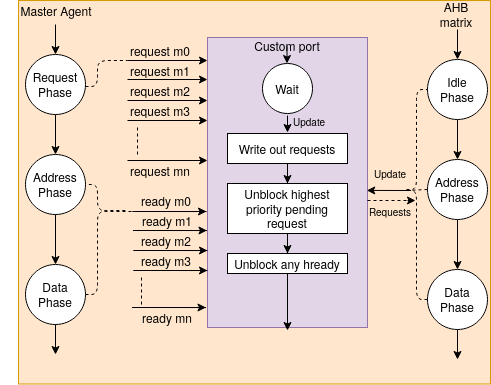
\includegraphics[width=5.5cm]{figs/ESL/port_diagram.png}
\caption{Illustration of port connection}\label{fig:cport}
\end{wrapfigure}

The port in figure \ref{fig:cport} is illustrated using the actual port directions in the ESL description, rather than the direction they symbolize. The inputs representing \textbf{HREADY} must be atomically unblocked which only happens when there is a pending handshake. To check for this the \textit{peek} function must be called, which is only available for reader ports. On the AHB matrix side the synchronization call to update the requests must always hand over control to the port by use of a wait function, which is only unconditionally called by use of a write port. When control is handed back to the AHB matrix the updated requests can be fetched from a shared port. 
\WKSAY{Consider if the port can include the payloads back and forth, although this is harder for burst due to the shared ports}

\subsubsection{Master agent}
\begin{wrapfigure}{l}{5.5cm}
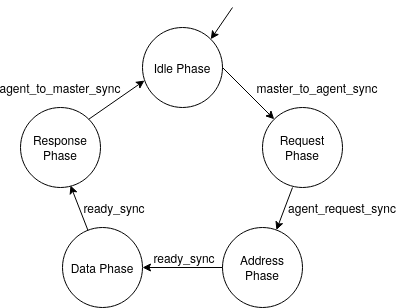
\includegraphics[width=5.5cm]{figs/ESL/mAgent_ESL.png}
\caption{master agent FSM}\label{fig:eafsm}
\end{wrapfigure}
The master agent is modeled at the ESL in a relatively simple manner using blocking ports to determine important states. All states from figure \ref{fig:rafsm} are deemed important states. They are all needed to communicate with the individual states of the bus matrix, or their masters. Transitions between the states are dependent on the synchronization signals alone, and all remaining interface signals are passed through shared ports. The generated properties are refined with minimal effort and proven to be a sound abstraction of the master agent RTL.  \\
\newline  

\subsubsection{Bus matrix}
The bus matrix has three main states as seen from figure \ref{fig:OC}. There is only one single communication with the emulated port in each of the three states. 
\begin{lstlisting}
   update_requests->try_write(true, sync, "idle_state");
   requests_in->get(reqs);
\end{lstlisting}

The sequence allows the emulated port to fetch most recent request from the master agents and update the shared port while the bus matrix is waiting. 
Even though requests are arbitrated within the port to ensure correct functionality, arbitration is again represented with an if then else cluster to represent this behavior in the properties. 
If there are no requests this state will loop, which is preferable to using a blocking write. The wait property associated with the blocking write is impossible to prove due to the possible immediate change of \textbf{HGRANTx}. \par
The payload of the highest priority request is stored in the compound \textit{AS\_regs}, and the bus proceeds to the address phase. (TODO: change bus state to phase, and master phase to state, more clear) 
The compound \textit{AS\_regs} represent the signals broadcast to the bus by the granted master, and is represented in the properties as visible registers. \par
In the address phase the values of \textit{AS\_regs} are stored in \textit{DS\_regs} and the operations in the previous phase are repeated, but without the possibility of a loop.
As seen from Fig.~\ref{fig:OC} the transition to the data phase is unconditional, as all slaves are required to be ready. The data phase is split into a series of substates as seen in Fig.~\ref{eslfsm}.
Since the master agent interface is represented using mostly shared ports, outputs must be written every clock cycle to successfully prove completeness. The properties generated for the shared outputs
are only defined at the right hook. In this case it is not sufficient for properties spanning more than one clock cycle. \par
The request sequence is again carried out, with the difference that it can transition to either of the three states. 
 

\subsection{Refining properties}
\label{sub:refine}
(gotta mention master agent state somewhere)
This section is an overview of the refinement of the properties, and the completeness proof. The interface to the master agents will be covered for both sides in parallel.
The signals \textbf{HREADY}, \textbf{HGRANTx} and \textbf{HBUSREQx} are represented with multiple macros in the property suite, which require explanation. 
\textit{update\_requests} represent all three signals functionally at the ESL, but the generated macros are not sufficient to prove completeness.
The macros needed to fullfil the requirements are listed in Fig.~\ref{fig_reqmac}, where superflous signals are omitted. 

\begin{figure}[hbt]
	\centering
	\begin{minipage}[t]{0.49\textwidth}
		\centering
                 \begin{enumerate}
                   \item \textit{reqs\_sig\_m(x)\_request}
                   \item \textit{update\_requests\_notify}
                   \item \textit{update\_requests\_sync}
                   \item \textit{bus\_to\_mAgent(x)\_sig\_hgrant}
                   \item \textit{m(x)\_grant}
                 \end{enumerate}
              
	\end{minipage}
	\begin{minipage}[t]{0.49\textwidth}
		\centering
		 \begin{enumerate}
                   \item \textit{mAgent\_request\_notify}
                   \item \textit{mAgent\_request\_sync}
                   \item \textit{bus\_ready\_sync}
                   \item \textit{bus\_to\_mAgent\_sig\_hgrant}
                 \end{enumerate}
              
	\end{minipage}
\caption{List of macros for request handling, with bus matrix on the left and master agent on the right}
\label{fig:reqmac}
\end{figure}

\newpage
Brief descriptions of the signals are given in table \ref{tab:reqmac}.

\begin{table}[hbt] 
  \label{tab:reqmac}
  \begin{tabular}{r p{10cm}} 
  \hline
  Matrix & Description \\
    \hline
  \textit{1.} & represents \textbf{HBUSREQx}, macro is determined as input in the completeness description \\
    \hline
  \textit{2.} & represents \textbf{HREADY} "or" (\textbf{HREADY} "and" \textbf{HGRANTx}). Macro is determined as output in the completeness description. This is sufficient to determine \textbf{HREADY}, but not \textbf{HGRANTx} \\
    \hline
  \textit{3.} & represents the "or" of all \textbf{HBUSREQx}, not part of completeness description, but added to table to provide consistency with 1. in agent. \\ 
    \hline
  \textit{4.} & represents \textbf{HGRANTx}, this signal is redefined as boolean and defined as output in the completeness description. \\
    \hline
  \textit{5.} & A function that calculates the current value of \textbf{HGRANTx} based on determined inputs and outputs \\
    \hline
  Agent & Description \\
    \hline
  \textit{1.} & represent \textbf{HBUSREQx}, defined as output in completeness description. \\
    \hline
  \textit{2.} & represents \textbf{HGRANT} "and" \textbf{HREADY}. Is not part of completeness description, but added to table to provide consistency with 2. in bus matrix. \\
    \hline
  \textit{3.} & represents \textbf{HREADY}, defined as input in completeness description \\
    \hline
  \textit{4.} & represent \textbf{HGRANTx}, redefined as boolean. Defined as input in completeness description. \\
    \hline  \end{tabular}
\caption{Description of macros for request handling}
\end{table}

The signals added to provide consistency are not strictly needed to pass any of hte completeness tests. It is rather a security measure to comply with the guidelines for working with clusters mentioned in 
Sec.~\ref{sub:clust}. Although the interface signals are not represented indentically on both sides, as long as the behavior is guaranteed within the emulated port it will not leave a gap in verification.

\subsubsection{Visible registers}
(only matrix)
The macros representing visible registers in the property suite are all variables in the ESL description which store values between the states. In this implementation none of the visible registers directly represent actual registers in the design. They represent input/outputs from/to masters and slaves, based on selection criteria. The selection criteria are generally the states of the master agents, or the conceptual state of the bus. 
\begin{itemize}
 \item \textit{AS\_regs}: Represents the subset of master agent outputs included in the payload, including \textbf{HTRANS} for the agent in its address state. If none it has default values.
 \item \textit{DS\_regs}: Either represents the subset of master agent outputs included in the payload for the agent in its data state. Or represents the output of the slave that has its out notify set. The address offset is effectively accounted for this way. If none apply it has default values
 \item \textit{resp}: Represents the response payload of the slave that has both its in notify and sync set the last 2 cycles. Otherwise it has default values.
 \item \textit{phase/nextphase}: Represents the main CSM of the bus matrix. Selected based on which state macro is true.
\end{itemize} 

(this all sucks but i definitely need to add that the completeness was initially done using only original I/O)


\section{Simulation}
\label{sec:sim}
Simulation models carrying out the same operations are designed for both abstraction layers. One of the main benefits of modeling hardware at the ESL is simulation speed, so a time comparison is carried out between the two layers. Designing two corresponding simulation models also offer some verification. 
The aim of PDD is to do away with RTL simulation all together, but when the ESL description is modeled after an existing hardware architecture it makes sense
to ensure that the two simulation models behave equivalent. \par
Master and slave dummies are connected to the bus matrix. The dummies perform simple operations to maintain a good overview of the operations. 
The masterdummy alternates between single read and writes. It increments the address by 10 every transaction, and the data by 1 every write. 
The simulation lasts for the duration of $10^6$ transfers, during which the address wraps around to 0 if it reaches the end of the slave address range. \par
Assertions are used to control that data is transmitted between the intended dummies. The slave dummy has no information about which master it is operated by. 
All masters can act independently from each other, and due to the arbitration it is not so simple to monitor from a top level perspective. It is an error prone
process and it is avoided. Instead, slaves also store their response in a map. The master asserts that the slave it intended to operate is the one that responds. VHDL offer no such high level functions for monitoring, so one part of the protocol is exploited. To recapitulate; A slave ignores \textbf{HWDATA} for reads, and masters ignore \textbf{HRDATA} for writes. This does not forbid any value being present on the signals for testing purposes. The master asserts
that the same data it writes to the slave is the same that returns. \par
Accessing the default slave does not increment the transfer count, so choosing a non continuous address range will affect the simulation time.  

\subsection{Starvation}
The downside of fixed priority arbitration is that there is no guarantee that every master is granted access to the bus. It is important that this feature is
accurately reflected in the ESL model. There are configurations of masters and slaves attempting to carry out a set of certain tasks where one or more master are never granted access to the bus. This type of configuration is useless and it defeats every purpose of fully verfifying at the ESL if this is not accurately reflected there. \par
The easiest example of starvation to observe is when all master dummies poll the bus. At the RTL, if the masters are requesting within the slave range a fourth master starves Whereas if they request outside the range it is the fifth master that starves. At the ESL on the other hand, it is the fourth master that starves
in either case. It is observed that this is due to an exactly three clock cycle delay, not present in the ESL simulation. This is impossible to model using "zero time" increments, but can be modeled by waiting exactly three times the minimum time increment after response from a master agent is received. This is provided that the minimum is above zero. \par
Will a full system still be represented correctly? maybe the fact that you dont know, if you have a system with many masters use RR.



\section{Generator}
\label{sec:generator}
The AHB system can be generated using a program implemented in C++, where the number of masters and slaves are required as input arguments. Allowed number of
masters and slaves are between 1 and 15. An ESL and RTL description, including testbenches are generated followed by a set of operation properties and completeness descriptions. Two short scripts are included which enable the property and completeness check to be carried out with just one command from the
command line. 

\subsubsection{Automatic property refinement}
The SystemC-PPA descriptions of the bus matrix and master agent are analyzed with the tool DeSCAM. The tool parses the SystemC-PPA and generates an abstract
model and properties. A plugin to the tool has been developed, which is tailored to the SystemC-PPA of the bus matrix and master agent. The plugin iterates 
over the abstract property set, and writes the property set to a file. The plugin inserts the appropriate signal names and logic in the macros as it is written.
 

\section{Experimental results}
\label{sec:results}



